\subsection{CodeBô: Design e avaliação de um puzzle game para o ensino de Estrutura de Dados}

O intuito deste projeto foi desenvolver um jogo digital chamado \textit{CodeBô}. Este é um jogo isométrico de \textit{puzzles} que se baseia na mecânica do \textit{lightBot}, mecânica esta que consiste em selecionar os movimentos do seu personagem para levá-lo de um local inicial até um local específico. O jogo \textit{CodeBô} utiliza essas mecânicas para ensinar conceitos como Pensamento Computacional, pilhas, filas e listas. \cite{de2025codebo}

\begin{figure}[H]
	\centering
	\caption{Captura de tela do jogo CodeBô}
	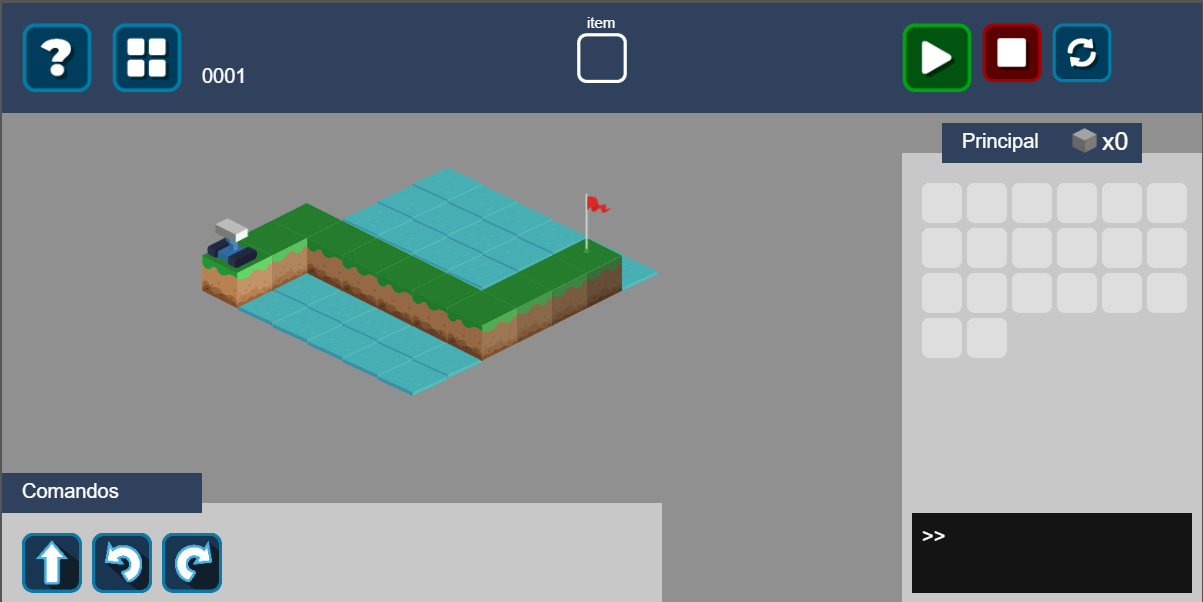
\includegraphics[width=0.8\textwidth]{images/codebo.png}
	\legend{Fonte: \cite{de2025codebo}}
	\label{fig:codebo}
\end{figure}


